\documentclass[11pt]{amsart}
\usepackage[margin=1in]{geometry}
\usepackage{graphicx}
\usepackage{siunitx}
\usepackage{amsmath,amsfonts,amsthm,amssymb,amsaddr}
\usepackage{hyperref}
\usepackage{fancyhdr}
\usepackage{multicol, caption}
\newenvironment{Figure}
  {\par\medskip\noindent\minipage{\linewidth}}
  {\endminipage\par\medskip}

\graphicspath{ {./images/} }

%\makeatletter
%\def\subsection{\@startsection{subsection}{3}%
%  \z@{.5\linespacing\@plus.7\linespacing}{.1\linespacing}%
%  {\normalfont\itshape}}
%\makeatother

\title{Lab Report}

\author{Joe Bentley}

\address{School of Physics and Astronomy \\ Tutor: Kevin Ralley}
\email{joebentley10@gmail.com}

\date{\today}

\begin{document}

\begin{abstract}
  In this paper the higgs data is analysed and we find the higgs with this statistical significance etc.
\end{abstract}

\maketitle

\newpage

\pagestyle{fancyplain}

\lhead{\footnotesize {Joe Bentley}}
\rhead{\footnotesize {Lab Report}}

\begin{multicols}{2}

\section{Theory}

\subsection{Four Momentum}

The four momentum is similar to the classical three component momentum except generalised to four dimensional space-time, so it also has an energy component. In the data supplied the four-momentum is given in the form $(p_x, p_y, p_z, E)$, where $p_z$ is aligned along the beam axis.

\subsection{Higgs Decay Channels}

The decay channel investigated in this experiment was the decay to a pair of photons through a top quark loop or W boson loop. This is significantly rarer than the other decay modes, but is used because the momenta of the photons can be measured much more accurately than other more massive particles, since the momenta of the photon is directly proportional to its energy, as the photon has no rest mass. (GET SOURCE)

The invariant mass is calculated using the relativistic equation for energy, in natural units this is given by,

\begin{equation}
  \label{eq:invariantmass}
  m_0^2 = E^2 - {|\mathbf{p}|}^2
\end{equation}

This is calculated in the parsing program by summing the four momenta from the event and then taking the scalar product of the resulting vector with itself. In Minkowski space-time has signature $(+, -, -, -)$ so this has the effect of the above equation. We then take the square root of the scalar product to find the invariant mass.

\section{PYTHIA}

The GPL-licensed PYTHIA was used to generate the collision data used in this experiment. \cite{pythia}

\section{Weighting}

The data given included $10,000$ signal events and $1,000,000$ background events. This is a much smaller ratio of signal to background events than would actually be observed in a real collider experiment, due to the low branching fraction of the $H \to \gamma\gamma$. The branching factor is the fraction of all particles which decay through a given decay mode, in this case the fraction of $H \to \gamma\gamma$ decays  over all Higgs decay modes. The theoretical ratio of the observed Higgs events to observed background events can be calculated by taking the ratio of the Higgs production cross section to the background cross section and multiplying it by the branching fraction of $H \to \gamma\gamma$,

\begin{equation}
  \label{eq:weighting}
  \frac{\text{num. H}}{\text{num. back}} = \frac{\sigma{\left(\text{H prod}\right)} \cdot B_f\left(H\to\gamma\gamma\right)}{\sigma{\left(\text{back}\right)}}
\end{equation}

where $\text{num. H}$ is the number of signal events, $\text{num. back}$ is the number of background events, $\sigma{\left(\text{H prod}\right)}$ is the Higgs production cross section, $\sigma{\left(\text{back}\right)}$ is the background cross section, and $B_f\left(H\to\gamma\gamma\right)$ is the branching fraction of Higgs to diphoton.


WHAT ARE THE NUMBERS? GIVE SOURCES FOR THEM


\section{Filters}

There are many more invariant masses from the background events than there are from the signal (Higgs) events. In fact after the weighting, there are roughly $100$ Higgs events to $100,000,000$ background events, so in the combined invariant mass histogram, with no filtering, the Higgs is practically invisible. Thus filtering is applied in the form of event selection to remove events which are clearly not Higgs events. There are a few kinds of filtering EXPLAIN THEM.

\subsection{Transverse Momenta Filtering}

The transverse momenta is the component of the momentum perpendicular to the beam axis. Since the $z$ component of the four-momentum, $p_z$ is aligned along the beam axis, the transverse momentum is given by $p_T = \sqrt{{p_x}^2 + {p_y}^2}$. This is filtered in two passes over both the signal and higgs events. Given an event with four momenta, first the event is discarded unless it has at least one four momentum above a given threshold, then all four momenta in the event below a certain threshold are discarded.

(JUSTIFICATION)

\subsection{Energy}

(Filter the energy, not sure if we will see results)

\subsection{Angular}

(Filter the difference in azimuthal angle and pseudorapidity squared)

\subsection{Final Selection}

Finally the two highest transverse momenta photons are chosen as the candidates to calculate the invariant mass from.

MENTION AZIMUTHAL SELECTION


\section{Optimisation of Filters}

To find the filter parameters that give the best chance of finding the Higgs we used the formula for the statistical significance of the higgs,

\begin{equation}
  \label{eq:significance}
  \Sigma = \frac{\text{no. signal}}{\sqrt{\text{no. signal} + \text{no. background}}}
\end{equation}

Each filter is applied to the signal (Higgs) and background events and then the above equation is used to find the statistical significance of the Higgs in those events by counting the number of signal and background events left after filtering. To find the best parameters to use for the filters a range of different parameters are tested, for example for the transverse momenta parameters are applied from $\SI{0}{\giga\electronvolt}$ to $\SI{700}{\giga\electronvolt}$ in steps of $\SI{100}{\giga\electronvolt}$, the value that gives the best statistical significance is then chosen as the current candidate for the best optimised value. Then the value is further optimised by taking the currently best optimised value and then checking the values around it, for example checking the value $\pm 10$ the current value. After checking a few times (HOW MANY TIMES?) the most optimum filter values to see the most Higgs event in the invariant mass histogram are attained.

INCLUDE SIGNIFICANCE PLOT!!!


\section{Invariant Mass Histogram}

The numpy library is used to generate an combined (signal and background) invariant mass histogram from the invariant masses calculated in the parsing script. The statistical significance of the signal (Higgs) is calculated using eq.~\ref{eq:significance} taken over a certain mass window (WHAT MASS WINDOW?!?), and gives a measure of how sure we can be that it is the Higgs in this mass range.

\begin{Figure}
  \centering
  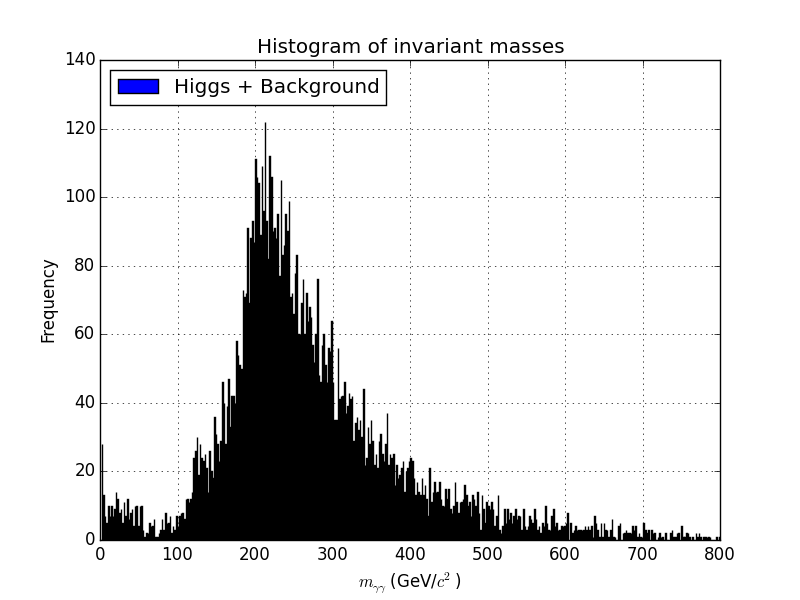
\includegraphics[width=\linewidth]{invmass}
  \captionof{figure}{Our awesome invariant mass plot yo!}
  \label{fig:invmass}
\end{Figure}

\end{multicols}

\bibliographystyle{plain}
\bibliography{citations}
\end{document}
